\chapter{Asynchronous Programming}

\section{The Need for Asynchronous Programming}

In modern system programming, efficiently managing concurrent operations is paramount. When deciding how to scale applications, we must fundamentally classify our workload into two categories: \textbf{CPU-bound} and \textbf{I/O-bound} tasks.

If an application is heavily CPU-bound (e.g., multiplying large matrices for AI inference), we rely on \textit{ideal parallelism}. We partition the mathematical workload across multiple threads—one for each physical CPU core—effectively reducing the total computational time. 

However, many modern applications, such as web servers or disk-crawlers, are heavily \textbf{I/O-bound}. They spend the vast majority of their lifecycle (often 99.9\%) waiting: waiting for a database to execute a query, waiting for the network to deliver a packet, or waiting for a disk to read a file block.

\subsection{The Cost of OS Threads}
A traditional approach to managing parallel I/O is allocating one thread per request. If 10,000 requests arrive, the system spawns 10,000 threads. But OS threads are heavily abstracted and come with significant overhead:
\begin{itemize}
    \item \textbf{Memory Footprint:} Each thread must pre-allocate a stack (often 1-2 MB). 10,000 threads immediately consume 10 to 20 GB of RAM, even if they are just idle.
    \item \textbf{Context Switching:} The OS uses a preemptive scheduler to switch between threads. Swapping registers, updating stack pointers, and invalidating the CPU caches/TLB for 10,000 threads introduces massive latency (often several milliseconds), effectively nullifying performance gains.
\end{itemize}

\begin{insightbox}
\textbf{The Asynchronous Paradigm} \\
We use OS threads to \textit{compute} in parallel, but we use asynchronous execution to \textit{wait} in parallel. Asynchronous programming allows a single thread to coordinate thousands of tasks simultaneously. It interleaves execution so that while one task is waiting for an I/O response, the thread can execute another task instead of blocking.
\end{insightbox}

\section{From Callbacks to Async/Await}

Historically, asynchronous behavior was achieved using \textit{callbacks} or \textit{continuations}. You would request an I/O operation and pass a function to be executed once the data arrived. While conceptually simple, this rapidly devolved into "callback hell" when chaining multiple operations, handling errors, or applying loops.

Rust elegantly solves this through the \texttt{async} and \texttt{await} keywords, which transform asynchronous logic into what looks like standard sequential code.

\begin{lstlisting}[language=Rust]
// A standard asynchronous function in Rust
async fn read_and_process(file_path: &str) -> Result<String, std::io::Error> {
    // We yield control back to the executor while waiting for the read
    let content = tokio::fs::read_to_string(file_path).await?;
    Ok(content.to_uppercase())
}
\end{lstlisting}

\begin{warningbox}
\textbf{Futures do nothing unless polled!} \\
Unlike in some other languages (like JavaScript), calling an \texttt{async fn} in Rust does \textbf{not} start executing the code immediately. Instead, it returns a \texttt{Future}—an inert representation of the computation. Execution only begins when you call \texttt{.await} on it, or explicitly hand it over to an executor.
\end{warningbox}

\section{The Future Trait and State Machines}

When the Rust compiler sees an \texttt{async fn}, it removes the \texttt{async} keyword and rewrites the return type to be an anonymous type implementing the \texttt{Future} trait. More importantly, it transforms the body of the function into a \textbf{state machine}. Every \texttt{.await} point becomes a state transition where the function can safely suspend and resume its execution.

The fundamental driving force behind asynchronous Rust is the \texttt{Future} trait:

\begin{lstlisting}[language=Rust]
pub trait Future {
    type Output;
    fn poll(self: Pin<&mut Self>, cx: &mut Context<'_>) -> Poll<Self::Output>;
}

pub enum Poll<T> {
    Ready(T),
    Pending,
}
\end{lstlisting}

\subsection{Polling and the Context}
When a future is awaited, it is repeatedly "polled". The \texttt{poll} method checks whether the data is ready to proceed to the next step of the state machine.
\begin{itemize}
    \item \texttt{Poll::Ready(T)}: The computation is complete, and it returns the result \texttt{T}.
    \item \texttt{Poll::Pending}: The future cannot make progress right now (e.g., the network packet hasn't arrived). It yields control back to the caller.
\end{itemize}

The \texttt{Context} argument contains a \texttt{Waker}. Before a future returns \texttt{Poll::Pending}, it registers this \texttt{Waker} with the underlying OS event loop. When the required event occurs (e.g., a file is loaded), the OS triggers the \texttt{Waker}, notifying the system that this specific future is ready to be polled again.

\begin{notebox}
\textbf{What is \texttt{Pin}?} \\
You may notice \texttt{Pin<\&mut Self>} in the signature. Because \texttt{async} functions compile down to state machines, they often contain internal references across \texttt{.await} points (self-referential structs). If the state machine were moved in memory, these pointers would be invalidated. \texttt{Pin} ensures the future cannot be moved in memory once polling begins.
\end{notebox}

\section{Executors and Cooperative Scheduling}

Rust itself does not include an asynchronous runtime; it only provides the \texttt{Future} trait and the state machine generator. To actually run asynchronous code, you must bring in an \textbf{Executor}. The most prominent executor in the Rust ecosystem is \textbf{Tokio}.

An executor acts as a \textbf{cooperative scheduler} operating in user space. It keeps a list of active tasks and repeatedly polls them.

\begin{figure}[h]
    \centering
    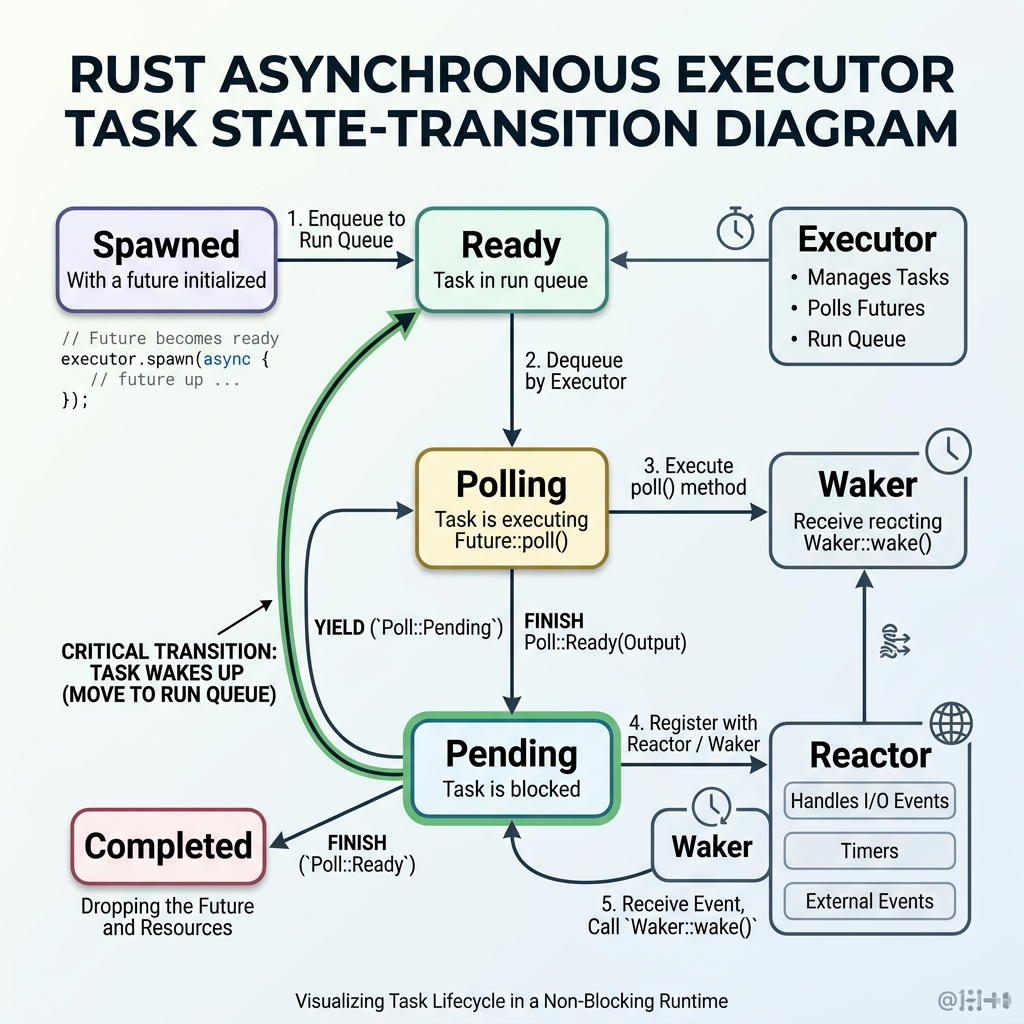
\includegraphics[width=\textwidth]{images/async_executor.png}
    \caption{Architecture of the Tokio Executor handling concurrent tasks.}
    \label{fig:async_executor}
\end{figure}

\subsection{Cooperative vs. Preemptive Scheduling}
OS threads use \textbf{preemptive scheduling}: the OS abruptly interrupts a running thread to give CPU time to another. 
Executors use \textbf{cooperative scheduling}: tasks are expected to voluntarily yield control back to the executor at \texttt{.await} points. If a task does not yield (e.g., it enters an infinite loop without an \texttt{.await}, or performs heavy synchronous CPU work), it "starves" the executor, preventing other asynchronous tasks on the same thread from running.

\subsection{Tokio and Task Spawning}
To execute independent concurrent operations in Tokio, we spawn \textbf{tasks}. A task is effectively a lightweight, user-space "green thread" managed by the Tokio executor.

\begin{lstlisting}[language=Rust]
#[tokio::main]
async fn main() {
    let task1 = tokio::spawn(async {
        // Do some async I/O
        tokio::time::sleep(std::time::Duration::from_secs(1)).await;
        "Task 1 done"
    });

    let task2 = tokio::spawn(async {
        // Do some other async I/O
        tokio::time::sleep(std::time::Duration::from_secs(2)).await;
        "Task 2 done"
    });

    // Wait for both tasks to complete
    let (res1, res2) = tokio::join!(task1, task2);
    println!("Results: {:?}, {:?}", res1, res2);
}
\end{lstlisting}

\begin{warningbox}
\textbf{Mutexes in Async Contexts} \\
Never hold a standard \texttt{std::sync::Mutex} lock across an \texttt{.await} point. Since tasks are cooperatively scheduled on shared executor threads, holding a standard OS thread lock across an \texttt{.await} can permanently deadlock the entire executor thread. If you must hold a lock across an \texttt{.await}, use an asynchronous lock like \texttt{tokio::sync::Mutex}, which yields the task instead of blocking the OS thread.
\end{warningbox}

\section*{End-of-Chapter Exam Questions}

\begin{exambox}
\textbf{Question 1: OS Threads vs. Async Tasks} \\
Describe the difference between preemptive scheduling (used by OS threads) and cooperative scheduling (used by Rust's async executors). Why is a cooperative approach more efficient for I/O bound workloads?

\textbf{Question 2: The Future Trait} \\
Explain the role of the \texttt{poll} method within the \texttt{Future} trait. What does it return, and what is the significance of the \texttt{Waker}?

\textbf{Question 3: Identifying Blocking Code} \\
Consider a Tokio runtime handling 10,000 asynchronous network connections. If one of the \texttt{async} tasks begins computing the 100,000th Fibonacci number using a synchronous \texttt{while} loop without \texttt{.await} points, what happens to the other connections? How should this be fixed?
\end{exambox}
